\documentclass{standalone}
\usepackage{tikz}
\usetikzlibrary{patterns, positioning}


\begin{document}
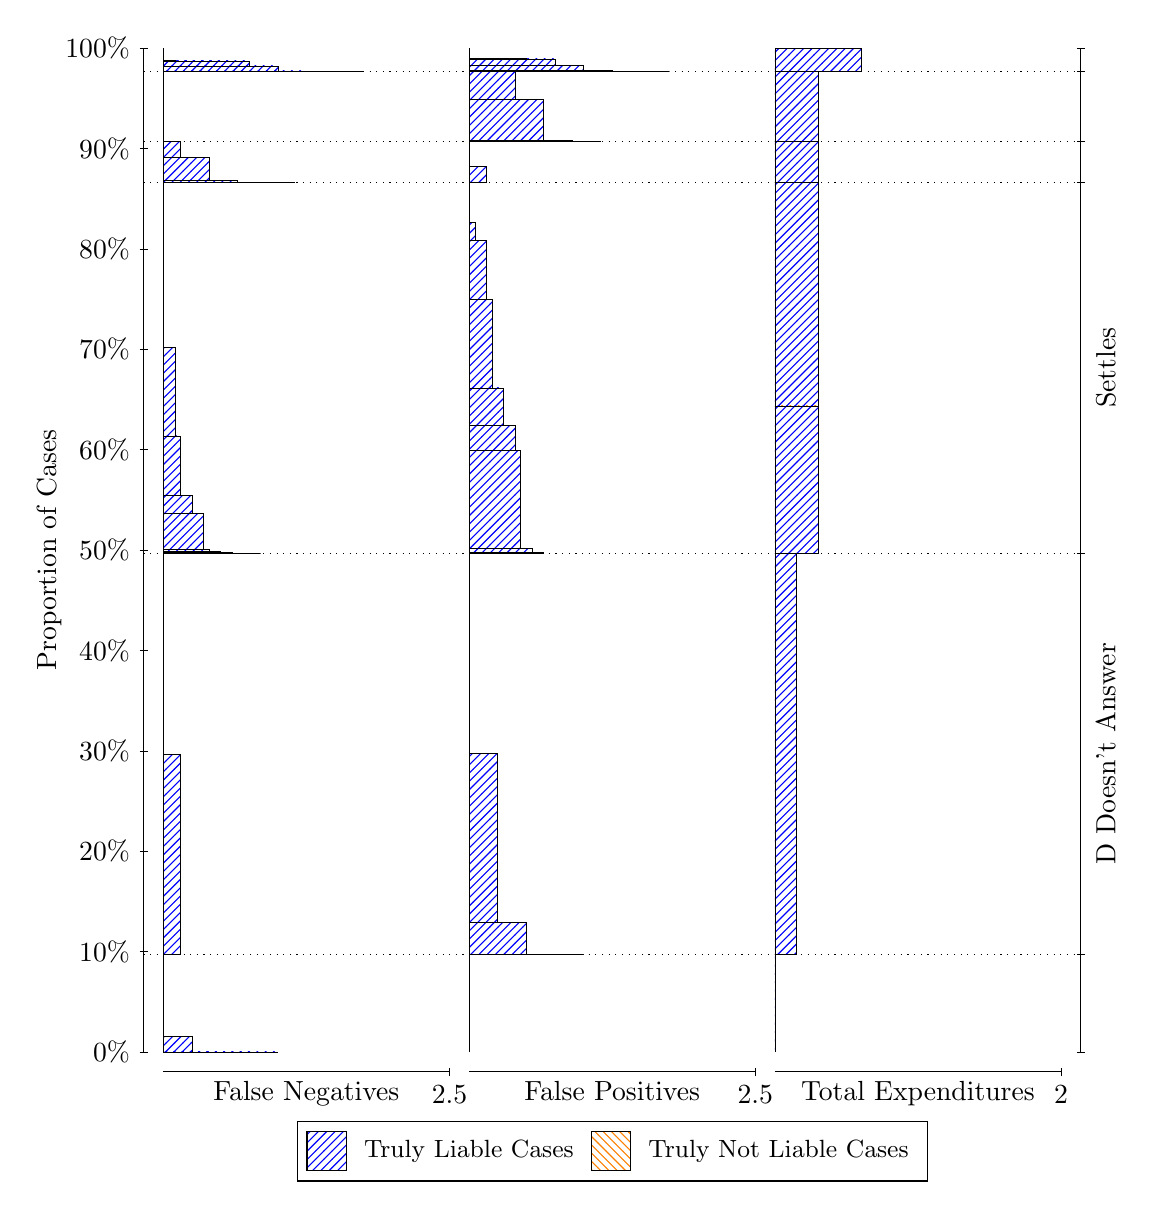
\begin{tikzpicture}
\draw[black, very thin] (1.5,1.75) -- (1.5,14.5);
\node[rotate=90, text=black, anchor=center] at (0.3, 8.125) {Proportion of Cases};
\draw[black, very thin] (1.45,1.75) -- (1.55,1.75);
\node[text=black, anchor=east] at (1.45, 1.75) {0\%};
\draw[black, very thin] (1.45,3.025) -- (1.55,3.025);
\node[text=black, anchor=east] at (1.45, 3.025) {10\%};
\draw[black, very thin] (1.45,4.3) -- (1.55,4.3);
\node[text=black, anchor=east] at (1.45, 4.3) {20\%};
\draw[black, very thin] (1.45,5.575) -- (1.55,5.575);
\node[text=black, anchor=east] at (1.45, 5.575) {30\%};
\draw[black, very thin] (1.45,6.85) -- (1.55,6.85);
\node[text=black, anchor=east] at (1.45, 6.85) {40\%};
\draw[black, very thin] (1.45,8.125) -- (1.55,8.125);
\node[text=black, anchor=east] at (1.45, 8.125) {50\%};
\draw[black, very thin] (1.45,9.4) -- (1.55,9.4);
\node[text=black, anchor=east] at (1.45, 9.4) {60\%};
\draw[black, very thin] (1.45,10.675) -- (1.55,10.675);
\node[text=black, anchor=east] at (1.45, 10.675) {70\%};
\draw[black, very thin] (1.45,11.95) -- (1.55,11.95);
\node[text=black, anchor=east] at (1.45, 11.95) {80\%};
\draw[black, very thin] (1.45,13.225) -- (1.55,13.225);
\node[text=black, anchor=east] at (1.45, 13.225) {90\%};
\draw[black, very thin] (1.45,14.5) -- (1.55,14.5);
\node[text=black, anchor=east] at (1.45, 14.5) {100\%};

\draw[black, very thin] (13.4,1.75) -- (13.4,14.5);
\draw[black, very thin] (13.35,1.75) -- (13.45,1.75);
\node[anchor=west] at (13.35, 1.75) {};
\draw[black, very thin] (13.35,2.9871) -- (13.45,2.9871);
\node[anchor=west] at (13.35, 2.9871) {};
\draw[black, very thin] (13.35,8.0854) -- (13.45,8.0854);
\node[anchor=west] at (13.35, 8.0854) {};
\draw[black, very thin] (13.35,12.793) -- (13.45,12.793);
\node[anchor=west] at (13.35, 12.793) {};
\draw[black, very thin] (13.35,13.312) -- (13.45,13.312);
\node[anchor=west] at (13.35, 13.312) {};
\draw[black, very thin] (13.35,14.206) -- (13.45,14.206);
\node[anchor=west] at (13.35, 14.206) {};
\draw[black, very thin] (13.35,14.5) -- (13.45,14.5);
\node[anchor=west] at (13.35, 14.5) {};

\draw[black, very thin, pattern color=blue, pattern=north east lines] (1.75,1.75) rectangle (3.2033,1.75);
\draw[black, very thin, pattern color=blue, pattern=north east lines] (1.75,1.75) rectangle (2.84,1.75);
\draw[black, very thin, pattern color=blue, pattern=north east lines] (1.75,1.75) rectangle (2.4767,1.7517);
\draw[black, very thin, pattern color=blue, pattern=north east lines] (1.75,1.7517) rectangle (2.1133,1.9526);
\draw[black, very thin, pattern color=orange, pattern=north west lines] (1.75,1.9526) rectangle (1.75,1.9526);
\draw[black, very thin, pattern color=blue, pattern=north east lines] (1.75,1.9526) rectangle (1.75,2.9871);
\draw[black, very thin, pattern color=blue, pattern=north east lines] (1.75,2.9871) rectangle (1.968,5.533);
\draw[black, very thin, pattern color=orange, pattern=north west lines] (1.75,5.533) rectangle (1.75,5.533);
\draw[black, very thin, pattern color=blue, pattern=north east lines] (1.75,5.533) rectangle (1.75,8.0854);
\draw[black, very thin, pattern color=blue, pattern=north east lines] (1.75,8.0854) rectangle (2.9853,8.0854);
\draw[black, very thin, pattern color=blue, pattern=north east lines] (1.75,8.0854) rectangle (2.84,8.0854);
\draw[black, very thin, pattern color=blue, pattern=north east lines] (1.75,8.0854) rectangle (2.6947,8.0854);
\draw[black, very thin, pattern color=blue, pattern=north east lines] (1.75,8.0854) rectangle (2.622,8.0989);
\draw[black, very thin, pattern color=blue, pattern=north east lines] (1.75,8.0989) rectangle (2.4767,8.1036);
\draw[black, very thin, pattern color=blue, pattern=north east lines] (1.75,8.1036) rectangle (2.3313,8.1363);
\draw[black, very thin, pattern color=blue, pattern=north east lines] (1.75,8.1363) rectangle (2.2587,8.588);
\draw[black, very thin, pattern color=blue, pattern=north east lines] (1.75,8.588) rectangle (2.1133,8.8215);
\draw[black, very thin, pattern color=blue, pattern=north east lines] (1.75,8.8215) rectangle (1.968,9.5755);
\draw[black, very thin, pattern color=blue, pattern=north east lines] (1.75,9.5755) rectangle (1.8953,10.695);
\draw[black, very thin, pattern color=orange, pattern=north west lines] (1.75,10.695) rectangle (1.75,10.695);
\draw[black, very thin, pattern color=blue, pattern=north east lines] (1.75,10.695) rectangle (1.75,12.793);
\draw[black, very thin, pattern color=blue, pattern=north east lines] (1.75,12.793) rectangle (3.4213,12.793);
\draw[black, very thin, pattern color=blue, pattern=north east lines] (1.75,12.793) rectangle (3.058,12.793);
\draw[black, very thin, pattern color=blue, pattern=north east lines] (1.75,12.793) rectangle (2.6947,12.815);
\draw[black, very thin, pattern color=blue, pattern=north east lines] (1.75,12.815) rectangle (2.3313,13.108);
\draw[black, very thin, pattern color=blue, pattern=north east lines] (1.75,13.108) rectangle (1.968,13.312);
\draw[black, very thin, pattern color=orange, pattern=north west lines] (1.75,13.312) rectangle (1.75,13.312);
\draw[black, very thin, pattern color=blue, pattern=north east lines] (1.75,13.312) rectangle (1.968,13.316);
\draw[black, very thin, pattern color=orange, pattern=north west lines] (1.75,13.316) rectangle (1.75,13.316);
\draw[black, very thin, pattern color=blue, pattern=north east lines] (1.75,13.316) rectangle (1.75,14.206);
\draw[black, very thin, pattern color=blue, pattern=north east lines] (1.75,14.206) rectangle (4.2933,14.206);
\draw[black, very thin, pattern color=blue, pattern=north east lines] (1.75,14.206) rectangle (3.93,14.206);
\draw[black, very thin, pattern color=blue, pattern=north east lines] (1.75,14.206) rectangle (3.5667,14.21);
\draw[black, very thin, pattern color=blue, pattern=north east lines] (1.75,14.21) rectangle (3.2033,14.272);
\draw[black, very thin, pattern color=blue, pattern=north east lines] (1.75,14.272) rectangle (2.84,14.336);
\draw[black, very thin, pattern color=blue, pattern=north east lines] (1.75,14.336) rectangle (2.622,14.336);
\draw[black, very thin, pattern color=blue, pattern=north east lines] (1.75,14.336) rectangle (2.4767,14.338);
\draw[black, very thin, pattern color=blue, pattern=north east lines] (1.75,14.338) rectangle (2.2587,14.338);
\draw[black, very thin, pattern color=blue, pattern=north east lines] (1.75,14.338) rectangle (2.2587,14.338);
\draw[black, very thin, pattern color=blue, pattern=north east lines] (1.75,14.338) rectangle (2.1133,14.338);
\draw[black, very thin, pattern color=blue, pattern=north east lines] (1.75,14.338) rectangle (1.8953,14.338);
\draw[black, very thin, pattern color=blue, pattern=north east lines] (1.75,14.338) rectangle (1.8953,14.343);
\draw[black, very thin, pattern color=orange, pattern=north west lines] (1.75,14.343) rectangle (1.75,14.343);
\draw[black, very thin, pattern color=blue, pattern=north east lines] (1.75,14.343) rectangle (1.75,14.5);
\draw[black, very thin, pattern color=orange, pattern=north west lines] (5.6333,1.75) rectangle (5.6333,1.75);
\draw[black, very thin, pattern color=blue, pattern=north east lines] (5.6333,1.75) rectangle (5.6333,2.9871);
\draw[black, very thin, pattern color=orange, pattern=north west lines] (5.6333,2.9871) rectangle (7.0867,2.9871);
\draw[black, very thin, pattern color=blue, pattern=north east lines] (5.6333,2.9871) rectangle (7.0867,2.9871);
\draw[black, very thin, pattern color=blue, pattern=north east lines] (5.6333,2.9871) rectangle (6.7233,2.9903);
\draw[black, very thin, pattern color=blue, pattern=north east lines] (5.6333,2.9903) rectangle (6.36,3.3946);
\draw[black, very thin, pattern color=blue, pattern=north east lines] (5.6333,3.3946) rectangle (5.9967,5.5395);
\draw[black, very thin, pattern color=blue, pattern=north east lines] (5.6333,5.5395) rectangle (5.6333,8.0854);
\draw[black, very thin, pattern color=orange, pattern=north west lines] (5.6333,8.0854) rectangle (6.578,8.0854);
\draw[black, very thin, pattern color=blue, pattern=north east lines] (5.6333,8.0854) rectangle (6.578,8.096);
\draw[black, very thin, pattern color=orange, pattern=north west lines] (5.6333,8.096) rectangle (6.4327,8.096);
\draw[black, very thin, pattern color=blue, pattern=north east lines] (5.6333,8.096) rectangle (6.4327,8.1423);
\draw[black, very thin, pattern color=orange, pattern=north west lines] (5.6333,8.1423) rectangle (6.2873,8.1423);
\draw[black, very thin, pattern color=blue, pattern=north east lines] (5.6333,8.1423) rectangle (6.2873,9.3948);
\draw[black, very thin, pattern color=blue, pattern=north east lines] (5.6333,9.3948) rectangle (6.2147,9.7038);
\draw[black, very thin, pattern color=blue, pattern=north east lines] (5.6333,9.7038) rectangle (6.0693,10.183);
\draw[black, very thin, pattern color=blue, pattern=north east lines] (5.6333,10.183) rectangle (5.924,11.303);
\draw[black, very thin, pattern color=blue, pattern=north east lines] (5.6333,11.303) rectangle (5.8513,12.057);
\draw[black, very thin, pattern color=blue, pattern=north east lines] (5.6333,12.057) rectangle (5.706,12.29);
\draw[black, very thin, pattern color=blue, pattern=north east lines] (5.6333,12.29) rectangle (5.6333,12.793);
\draw[black, very thin, pattern color=orange, pattern=north west lines] (5.6333,12.793) rectangle (5.8513,12.793);
\draw[black, very thin, pattern color=blue, pattern=north east lines] (5.6333,12.793) rectangle (5.8513,12.997);
\draw[black, very thin, pattern color=blue, pattern=north east lines] (5.6333,12.997) rectangle (5.6333,13.312);
\draw[black, very thin, pattern color=orange, pattern=north west lines] (5.6333,13.312) rectangle (7.3047,13.312);
\draw[black, very thin, pattern color=blue, pattern=north east lines] (5.6333,13.312) rectangle (7.3047,13.312);
\draw[black, very thin, pattern color=blue, pattern=north east lines] (5.6333,13.312) rectangle (6.9413,13.326);
\draw[black, very thin, pattern color=blue, pattern=north east lines] (5.6333,13.326) rectangle (6.578,13.851);
\draw[black, very thin, pattern color=blue, pattern=north east lines] (5.6333,13.851) rectangle (6.2147,14.202);
\draw[black, very thin, pattern color=blue, pattern=north east lines] (5.6333,14.202) rectangle (5.8513,14.206);
\draw[black, very thin, pattern color=orange, pattern=north west lines] (5.6333,14.206) rectangle (8.1767,14.206);
\draw[black, very thin, pattern color=blue, pattern=north east lines] (5.6333,14.206) rectangle (8.1767,14.206);
\draw[black, very thin, pattern color=orange, pattern=north west lines] (5.6333,14.206) rectangle (7.8133,14.206);
\draw[black, very thin, pattern color=blue, pattern=north east lines] (5.6333,14.206) rectangle (7.8133,14.206);
\draw[black, very thin, pattern color=orange, pattern=north west lines] (5.6333,14.206) rectangle (7.45,14.206);
\draw[black, very thin, pattern color=blue, pattern=north east lines] (5.6333,14.206) rectangle (7.45,14.213);
\draw[black, very thin, pattern color=orange, pattern=north west lines] (5.6333,14.213) rectangle (7.0867,14.213);
\draw[black, very thin, pattern color=blue, pattern=north east lines] (5.6333,14.213) rectangle (7.0867,14.279);
\draw[black, very thin, pattern color=blue, pattern=north east lines] (5.6333,14.279) rectangle (6.7233,14.363);
\draw[black, very thin, pattern color=blue, pattern=north east lines] (5.6333,14.363) rectangle (6.36,14.368);
\draw[black, very thin, pattern color=orange, pattern=north west lines] (5.6333,14.368) rectangle (6.142,14.368);
\draw[black, very thin, pattern color=blue, pattern=north east lines] (5.6333,14.368) rectangle (6.142,14.368);
\draw[black, very thin, pattern color=blue, pattern=north east lines] (5.6333,14.368) rectangle (5.9967,14.368);
\draw[black, very thin, pattern color=orange, pattern=north west lines] (5.6333,14.368) rectangle (5.7787,14.368);
\draw[black, very thin, pattern color=blue, pattern=north east lines] (5.6333,14.368) rectangle (5.7787,14.37);
\draw[black, very thin, pattern color=orange, pattern=north west lines] (5.6333,14.37) rectangle (5.6333,14.37);
\draw[black, very thin, pattern color=blue, pattern=north east lines] (5.6333,14.37) rectangle (5.6333,14.5);
\draw[black, very thin, pattern color=orange, pattern=north west lines] (9.5167,1.75) rectangle (9.5167,1.75);
\draw[black, very thin, pattern color=blue, pattern=north east lines] (9.5167,1.75) rectangle (9.5167,2.9871);
\draw[black, very thin, pattern color=orange, pattern=north west lines] (9.5167,2.9871) rectangle (9.7892,2.9871);
\draw[black, very thin, pattern color=blue, pattern=north east lines] (9.5167,2.9871) rectangle (9.7892,8.0854);
\draw[black, very thin, pattern color=orange, pattern=north west lines] (9.5167,8.0854) rectangle (10.062,8.0854);
\draw[black, very thin, pattern color=blue, pattern=north east lines] (9.5167,8.0854) rectangle (10.062,9.9558);
\draw[black, very thin, pattern color=orange, pattern=north west lines] (9.5167,9.9558) rectangle (10.062,9.9558);
\draw[black, very thin, pattern color=blue, pattern=north east lines] (9.5167,9.9558) rectangle (10.062,12.793);
\draw[black, very thin, pattern color=orange, pattern=north west lines] (9.5167,12.793) rectangle (10.062,12.793);
\draw[black, very thin, pattern color=blue, pattern=north east lines] (9.5167,12.793) rectangle (10.062,13.312);
\draw[black, very thin, pattern color=orange, pattern=north west lines] (9.5167,13.312) rectangle (10.062,13.312);
\draw[black, very thin, pattern color=blue, pattern=north east lines] (9.5167,13.312) rectangle (10.062,14.206);
\draw[black, very thin, pattern color=orange, pattern=north west lines] (9.5167,14.206) rectangle (10.607,14.206);
\draw[black, very thin, pattern color=blue, pattern=north east lines] (9.5167,14.206) rectangle (10.607,14.5);
\draw[black, dotted] (1.5,2.9871) -- (13.4,2.9871);
\draw[black, dotted] (1.5,8.0854) -- (13.4,8.0854);
\draw[black, dotted] (1.5,12.793) -- (13.4,12.793);
\draw[black, dotted] (1.5,13.312) -- (13.4,13.312);
\draw[black, dotted] (1.5,14.206) -- (13.4,14.206);
\draw[black, very thin] (1.75,1.5) -- (5.3833,1.5);
\node[text=black, anchor=north] at (3.5667, 1.5) {False Negatives};
\draw[black, very thin] (5.3833,1.45) -- (5.3833,1.55);
\node[text=black, anchor=north] at (5.3833, 1.45) {2.5};

\draw[black, very thin] (5.6333,1.5) -- (9.2667,1.5);
\node[text=black, anchor=north] at (7.45, 1.5) {False Positives};
\draw[black, very thin] (9.2667,1.45) -- (9.2667,1.55);
\node[text=black, anchor=north] at (9.2667, 1.45) {2.5};

\draw[black, very thin] (9.5167,1.5) -- (13.15,1.5);
\node[text=black, anchor=north] at (11.333, 1.5) {Total Expenditures};
\draw[black, very thin] (13.15,1.45) -- (13.15,1.55);
\node[text=black, anchor=north] at (13.15, 1.45) {2};


\node[text=black, centered, rotate=90] at (13.72, 5.5362) {D Doesn't Answer};
\node[text=black, centered, rotate=90] at (13.72, 10.439) {Settles};




\draw (7.449999999999999,1.5) node[draw=none] (baseCoordinate) {};
\begin{scope}[align=center]
        \matrix[scale=0.5, draw=black, below=0.5cm of baseCoordinate, nodes={draw}, column sep=0.1cm]{
            \node[rectangle, draw, minimum width=0.5cm, minimum height=0.5cm, pattern color=blue, pattern=north east lines] {}; &
            \node[draw=none, font=\small, text=black] (B) {Truly Liable Cases}; &
            \node[rectangle, draw, minimum width=0.5cm, minimum height=0.5cm, pattern color=orange, pattern=north west lines] {}; &
            \node[draw=none, font=\small, text=black] (B) {Truly Not Liable Cases}; \\
            };
\end{scope}

\end{tikzpicture}
\end{document}